\documentclass[runningheads]{llncs}
\usepackage[T1]{fontenc}
\usepackage{graphicx}
\usepackage{amsmath}
\usepackage{booktabs}
\usepackage{xurl}
\usepackage[hidelinks]{hyperref}
\usepackage{color}
\renewcommand\UrlFont{\color{blue}\rmfamily}
\urlstyle{rm}
\providecommand{\Description}[1]{}

\newcommand{\BA}{\ensuremath{\mathrm{BA}_2}}
\DeclareRobustCommand{\WRITE}[1]{\textbf{[WRITE #1]}}

\begin{document}

\title{Answer, Clarify or Refuse? A Locked, Run-Once Evaluation on Real Vietnamese Citizen Questions, with a Rule-Layer Case Study}
\titlerunning{Answer, Clarify or Refuse on Real Citizen Questions}

\author{Hoang Nhan Trinh\inst{1}\orcidID{0009-0003-1961-9022} \and
Viet Hung Nguyen\inst{1}\orcidID{0009-0006-5603-6143} \and
Le Thien Dan Pham\inst{1}\orcidID{0009-0006-3191-0965} \and
Long Truong\inst{2}\orcidID{0009-0007-0928-2015}\thanks{Corresponding author.} \and
Anh Duy Bui\inst{2} \and
Ngoc Minh Chau Hoang\inst{2}}

\authorrunning{H. N. Trinh et al.}

\institute{Department of Artificial Intelligence, FPT University, Ho Chi Minh City, Vietnam\\
\email{hoangnhan070206@gmail.com}, \email{hung2272006@gmail.com}, \email{phamlethiendan1@gmail.com}
\and
Faculty of Software Engineering, FPT University, Ho Chi Minh City, Vietnam\\
\email{longt5@fpt.edu.vn}, \email{anhduy290605@gmail.com}, \email{chauhnmss181219@fpt.edu.vn}}

\maketitle

\begin{abstract}

{An e-gov procedure assistant faces three choices: answer / clarify / refuse. We introduce a locked, run-once protocol with pre-test labeling, hashing, selection criteria and key comparisons. We apply it to an assistant for 542 commune/ward-level Vietnamese procedures. We also introduced 958 real-world questions from two public-service portals (public ID, source pointer, labels, no raw-text distribution). On the same frozen system: behavior accuracy decreased from 77.2\% (team's own test set) to 56.5\% (real-world questions). 79\% of citizen questions required refusal. The AI-assisted rule layer raises test 1 (T1) \BA{} (balanced
accuracy) by +0.167 [0.095, 0.240], mainly through accurate refusals.  End-to-end correct answers (E2E) increased from 19 to 35 out of 59. On test 2 (T2), declared comparison (base vs A2+B) raised \BA{} by +0.158 [0.009, 0.304]. With second-rule layer, dev set shows +25 correct behavior decisions and 0 errors compared with A, but on T2, no gain was detected +0.046 [-0.048, 0.143]. The reranker, LLM reader, two learned gates did not detectably improve \BA{} or E2E. The RAG pipeline (self-determined by LLM) was no better than the always-refuse strategy. The minimum detectable effect (MDE) ranged from 0.04-0.13 (T1) and 0.13-0.21 (T2). Only 6 and 7 questions were labeled ``clarify'' across two test sets; leaving clarification virtually unevaluated. On T2: the always-refuse strategy provides at least the same utility as any configuration when an incorrect answer carries a cost at least one-fourth the value of a correct answer.}

\keywords{Abstention \and Question answering \and Evaluation protocol \and Vietnamese \and E-government.}
\end{abstract}

\section{Introduction}

{Reliable language technologies are essential for e-government. Knowing when not to answer is often more critical than finding information. There are many routine procedures at the commune level in Vietnam, including civil status, residence, ID cards, certified copies and social benefits. Each is described in detail on the National Public Service Portal ~\cite{dvcportal}. However, citizens frequently include some greetings, family background, a letter-like message, abbreviations or missing diacritics. Many ask about their own circumstances: a complaint, fine, submitted file status or police officer benefits. This causes problems due to providing incorrect advice based on the procedure which wasting citizens' time and eroding trust in service ~\cite{kaplan2026,samson2026}.}

{In order to retrieve an answer, model must determine answering when a single possible process, clarifying when multiple fit or refusing when out of scope. Knowing when to refuse is a known weakness with LMs ~\cite{wen2025,kamath2020}. Queries that are out of scope can cause issues with intent classifiers ~\cite{larson2019}. To our knowledge previous works on Vietnamese public service QA have evaluated answerable questions only ~\cite{phamduy2023}. Experimental evaluations face three common pitfalls: team-authored test questions, repeated test reuse during tuning ~\cite{dwork2015,gorman2019}, due to small answerable sample sizes insufficient causing underpowered comparisons. We study a commune-level assistant covering communes, wards and special zones, deployed locally on a single machine. Our research questions are:}
\begin{itemize}

\item[\textbf{RQ1}]
{How do the shares of answer, clarify and refuse differ between real citizens and team-written regression and how does this difference affect measured quality on the same frozen system?}

\item[\textbf{RQ2}]
{Under a locked, run-once protocol, to what extent does an AI-assisted rule layer improve performance on sequentially locked test sets? Which components contribute to this improvement? And does this effectiveness persist when moving to a second round of rules?}

\item[\textbf{RQ3}]
{Under the same protocol, how do a reranker, a small local LLM reader, learned refusal gates and an LLM-decided RAG pipeline compare, and what effect sizes are detectable with 59 and 21 answerable test questions?}

\item[\textbf{RQ4}]
{If wrong answers are costlier than refusals, can any configuration beat always-refuse on real traffic?}
\end{itemize}

{There are three contributions: (1) A scope-decision protocol for applied assistants (Sect.~\ref{sec:protocol}), executed twice and documented per commit; reporting paired intervals, MDE, equivalence margins, and cost-weighted utility beyond significance testing; (2) a benchmark of 958 labeled real-citizen questions (Sect.~\ref{sec:data}) releasing IDs, source pointers, labels, and per-question decisions across 18 configurations; (3) Case study of an AI-assisted rule layer, compared with four alternatives (Sects.~\ref{sec:systems}--\ref{sec:discussion}).}

\section{Related Work}

\subsubsection{Vietnamese Public-Service and Legal QA.}

{For public-service questions, Pham Duy and Le Thanh~~\cite{phamduy2023} locate legal text with BM25+, a PhoBERT-based encoder~~\cite{nguyen2020phobert} and a final cross-encoder. ViGPTQA~~\cite{vigptqa2023} adapts Vietnamese LLMs to question answering (QA), including law. Pham et al.~~\cite{hien2025} add an LLM to legal retrieval and refer out-of-scope questions to legal experts, an untested step. ALQAC 2021~~\cite{alqac2021} benchmarks retrieval and answering over Vietnamese law. Closest to us, VietPSLM~~\cite{le2025vietpslm} pairs a small language model with public-service QA resources. To our knowledge, none tests answering, clarifying and refusing on citizens' own questions, with a locked protocol.
}

\subsubsection{Abstention and Out-of-Scope Detection.}

{Abstaining cuts risk but also coverage~~\cite{elyaniv2010,geifman2017}
, pricing errors against rejections~~\cite{chow1970}. Post hoc, maximum softmax probability~~\cite{hendrycks2017} flags errors and out-of-distribution inputs. QA calibrators guide abstention under domain shift~~\cite{kamath2020}, whereas out-of-scope queries trip intent classifiers~~\cite{larson2019}. LLM abstention has a survey~~\cite{wen2025}, and clarifying is a third path~~\cite{aliannejadi2019}.}

\subsubsection{Who Decides.}

{The organizing question is who decides. In RAG~~\cite{lewis2020} and self-reflective RAG~~\cite{asai2024} the model decides; in guardrails, rails written by developers do~~\cite{rebedea2023}. Rules remain common in industrial information extraction~~\cite{chiticariu2013}. An e-government pipeline escalates to humans~~\cite{kaplan2026}, and a benchmark scores answering and admitting ignorance separately~~\cite{samson2026}.}

\subsubsection{Evaluation Practice and LLM-Assisted Labels.}

{NLP has seen calls for preregistration~~\cite{vanmiltenburg2021}. One split can flip conclusions~~\cite{gorman2019}, tuning effort merits reporting~~\cite{dodge2019}, and adaptive holdout reuse overstates accuracy~~\cite{dwork2015}. LLMs can annotate better than crowd workers~~\cite{gilardi2023}, if validated~~\cite{pangakis2023,reiss2023}, a caveat for our LLM-assisted labels.}

\section{Task and Benchmark}\label{sec:data}

\subsubsection{Task.}

{The system returns an answer with a procedure ID, a clarification with candidate procedures, or a reasoned refusal, following written annotation guidelines. Answer is assigned when one clear commune-level procedure (or equivalent pair) is needed. Clarification is requested when multiple different procedures can be used or if only province-specific versions exist but no province is mentioned. Refusal covers missing or out-of-scope procedures, submitted-file status, complaints, petitions, legal questions, penalties, police internal matters and non-administrative requests.}

\subsubsection{Data.}

{We retrieved 1517  administrative procedures from the National Public Service Portal (NPSP) ~\cite{dvcportal} on 13 October 2026 from public JSON endpoints. Access was made at two requests per second without logging in, and 542 were at commune level. Questions were gathered from public Hugging Face datasets Binh Dinh ~\cite{hfdvc} and the Ministry of Public Security (MPS) ~\cite{hfmps}. Personal data were masked, duplicates removed and sentences shorter than four words dropped. We also dropped 266 earlier to design clarification rules. The resulting dataset contained 1490 questions (753 from MPS, 737 from Binh Dinh). Sampling with a fixed seed produced a dev of 282 questions (55 answer, 7 clarify, 220 refuse). Sampling covered random and topical strata, with topical commune-level keywords fixed before inspecting outputs. Test set (T1) contained 348 samples (120 random samples, 228 topic samples). Then reduce T1 to 313 samples (59 answer, 6 clarify, 248 refuse). Only T1 random stratum has 102 questions (11 answer, 1 clarify, 90 refuse). This test set contained 11 near duplicate questions from dev and 35 meaning unclear without context or non-questions that were skipped. Finally, T2 drew upon 814 unused questions, excluding all dev and T1. T2 also excluding four format checking questions and 25 near-duplicates not sampled in dev or T1 sets. Shuffled once and frozen, 400 first label questions yielded 363 random samples after skipping 37 questions as truncated or unintelligible (21 answer, 7 clarify, 335 refuse) (92\% refusing).}

\subsubsection{Labels and AI Involvement.}

{With labeling tool for dev and T1 we used Claude Opus 5.5 (Anthropic) under the guideline. This assistant later wrote rule layer and ran two passes for dev labels. Disagreements were resolved using the assistant's proposals, subject to project lead approval. The assistant read all 348 questions while labeling. Labels were then SHA-256-hashed and committed before any changes. Rules were derived solely from dev and procedure and T1 was never reopened. In the second pass, Gemini 4 Argon (Google) proposed labels for 100 randomly sampled T1 questions. Each question was reviewed by the lead without knowledge of the initial labeling. He knew only the proportion of each class. There were 91 questions retained across both passes, of which 79 agreed. Cohen's $\kappa = 0.685$ ~\cite{cohen1960} with  95\% bootstrap [0.55--0.82]. In disagreement, we have 8 out of 12 between answer and clarify. For the binary refuse versus non-refuses distinction, 87 show agreement with Cohen's $\kappa =0.887$ [0.767, 0.974]. This agreement reflects two LLM-assisted annotation processes, not independent humans. First-pass labels were retained as the official labels. In T2, Gemini 4 Argon proposed labels and then lead checked one by one. Guideline in T2 introduced two additional clarifications (petitions to refuse and two closely equivalent procedures yield single answer label). Lead only knew rule types to be added, not the specific content or even the output on T2.}

\subsubsection{Team-Written Set and Release.}

{For comparison, team's regression set contained 553 questions in blind part. There were 35 dropped across runs because gold procedure absent from snapshot. Those included 25 answer and 10 clarify. The remaining 518 comprised 384 answer questions (381 with gold procedure), 76 clarify and 58 refuse. Refusals accounted for 11\%. Release details are provided in Sect.~\ref{sec:conclusion}.}

\section{Evaluation Protocol}\label{sec:protocol}

\subsection{Locks, Single Runs and Declared Comparisons}

{Test sets were labeled and locked (SHA-256 hash and git commit) before writing code they tested. Rules and thresholds used dev data only;selection rules were written down before each run; code was frozen and each configuration ran once. No test sets guided design choices because selection on test data inflates estimates ~\cite{dwork2015}. T1 was locked at \texttt{7e78438} on 24 October; round-1 code and selection rules were frozen at \texttt{b7010d1}, running once at \texttt{7d199f3} on 25 October. Only after round 1, T1 was merged into dev (yielding 595 questions) for round 2. T2 order and labels were committed at \texttt{5499d0f} and \texttt{a79ec5f}; round-2 code and its plan were frozen at \texttt{88cabd6}, running once that evening.}

{The selection rule was documented before each run. We selected the dev configuration with the highest \BA{} subject to E2E $\geq$ the rule layer, breaking ties by E2E. A+B was selected for round 1 and A2+B for round 2; on dev, A2+B tied A2 at \BA{}=0.916 but won the E2E tie-break (88 vs 87 answers). This estimate is optimistic, as the rules were tuned on these same questions. The prespecified round-1 comparisons were base against each variant and the selected configuration using Wilson intervals. Round 2 prespecified three main McNemar tests: A+B vs A2+B, base vs A2+B and A2+B vs R, other comparisons were descriptive.}

{There were three protocol deviations. (i) The RAG baseline (R) was added after running T1. Its prompt was chosen on dev and frozen at \texttt{65b55af} before its one T1 run. Comparisons with R were descriptive on T1, where R was prespecified for T2. (ii) Post-hoc ablations alongside learned gates were evaluated after internal review with frozen code. (iii) The team-written set was initially run using the pre-freeze tree at \texttt{7e78438}, then run again on 27 October using the round two frozen code without round-2 rule (\texttt{92b0d6e}; \texttt{4bb4cfc}). The same decisions were made for all 518 questions.}

\subsection{Metrics and Statistics}\label{sec:metrics}

{We measure behavior accuracy by the percentage of three-way decisions that were made correctly. However because always-refuse reached 79.2\% on T1, 92.3\% on T2, we instead measure two-class balanced accuracy (\BA{}) ~\cite{brodersen2010} as given in Eq.~\eqref{eq:ba2}. A decision is correct if it agrees with the label. Even if the retrieved procedure is incorrect, a decision of ``answer'' counts as correct. Clarify-labeled examples are excluded from \BA{} as there are only 6 and 7 in T1 and T2 respectively. Deciding to clarify on any other query is penalized as an error.}
\begin{equation}
\BA = \frac{1}{2}\left(\frac{\mathit{TP}_\mathrm{ans}}{N_\mathrm{ans}} + \frac{\mathit{TP}_\mathrm{ref}}{N_\mathrm{ref}}\right)\label{eq:ba2}
\end{equation}

{Because \BA{} does not assess  whether the retrieved procedure is correct, we also report co-primary answering metrics. E2E is the number of questions answered with the correct top-1 procedure. Precision measures what percentage of all answers are correct. Top-1 measures what percentage of answer questions have the correct top-1 procedure. In deployment, coverage represents the proportion of questions answered. Selective risk is $1-\text{precision}$ ~\cite{elyaniv2010}. We measure the error-reject trade-off in terms of utility ~\cite{chow1970}, scaled per 100 questions in Eq.~\eqref{eq:utility}. Refusals and clarifications yield 0, giving always-refuse $U=0$. The break-even cost given by $c^*$ is the maximum wrong-answer cost below which a configuration beats always-refuse.}
\begin{equation}
U(c) = 100\,\frac{\mathit{correct} - c\cdot\mathit{wrong}}{n}, \qquad c^* = \frac{\mathit{correct}}{\mathit{wrong}}\label{eq:utility}
\end{equation}
 
{Wilson 95\% CI ~\cite{wilson1927} are reported. Pairwise comparisons are made using exact two-sided McNemar tests ~\cite{mcnemar1947,dietterich1998}. Exact McNemar tests were pre-specified only in round 2, round-1 tests were selected at reporting. We also calculate paired bootstrap 95\% percentile confidence intervals for $\Delta$ \BA{} $\Delta E2E$ and using 4000 bootstrap samples after both runs. No adjustment was made for multiple testing. Any confirmatory statements are based on those pre-specified. Minimum detectable effects (80\% power) ~\cite{connor1987} are also reported. The equivalence margin is the smallest value of $m$ for which the 90\% interval lies within $\pm m$. This corresponds to two one-sided tests at $\alpha=0.05$ ~\cite{schuirmann1987}. All values of $p$ should be reported to three decimal places for $p\geq0.001$, otherwise to one significant figure.}

\section{Systems Under Test}\label{sec:systems}

\subsection{Base System and AI-Assisted Rule Layer}

{The base system (Fig.~\ref{fig:pipeline}) makes no LLM-based decisions. Instead, it normalizes question segments and ranks procedures using syllable IDF weights, applying a 0.35 penalty for diacritics mismatch. A candidate procedure is accepted when score $\geq 0.55$ and coverage $\geq 0.5$. Coverage is the share of question-term weights covered by the procedure name. A policy module ensures alignment with the data. Answering is done automatically by pulling information from the procedures. LLM rewriting is disabled in all runs.}

\begin{figure}[tbp]
\centering
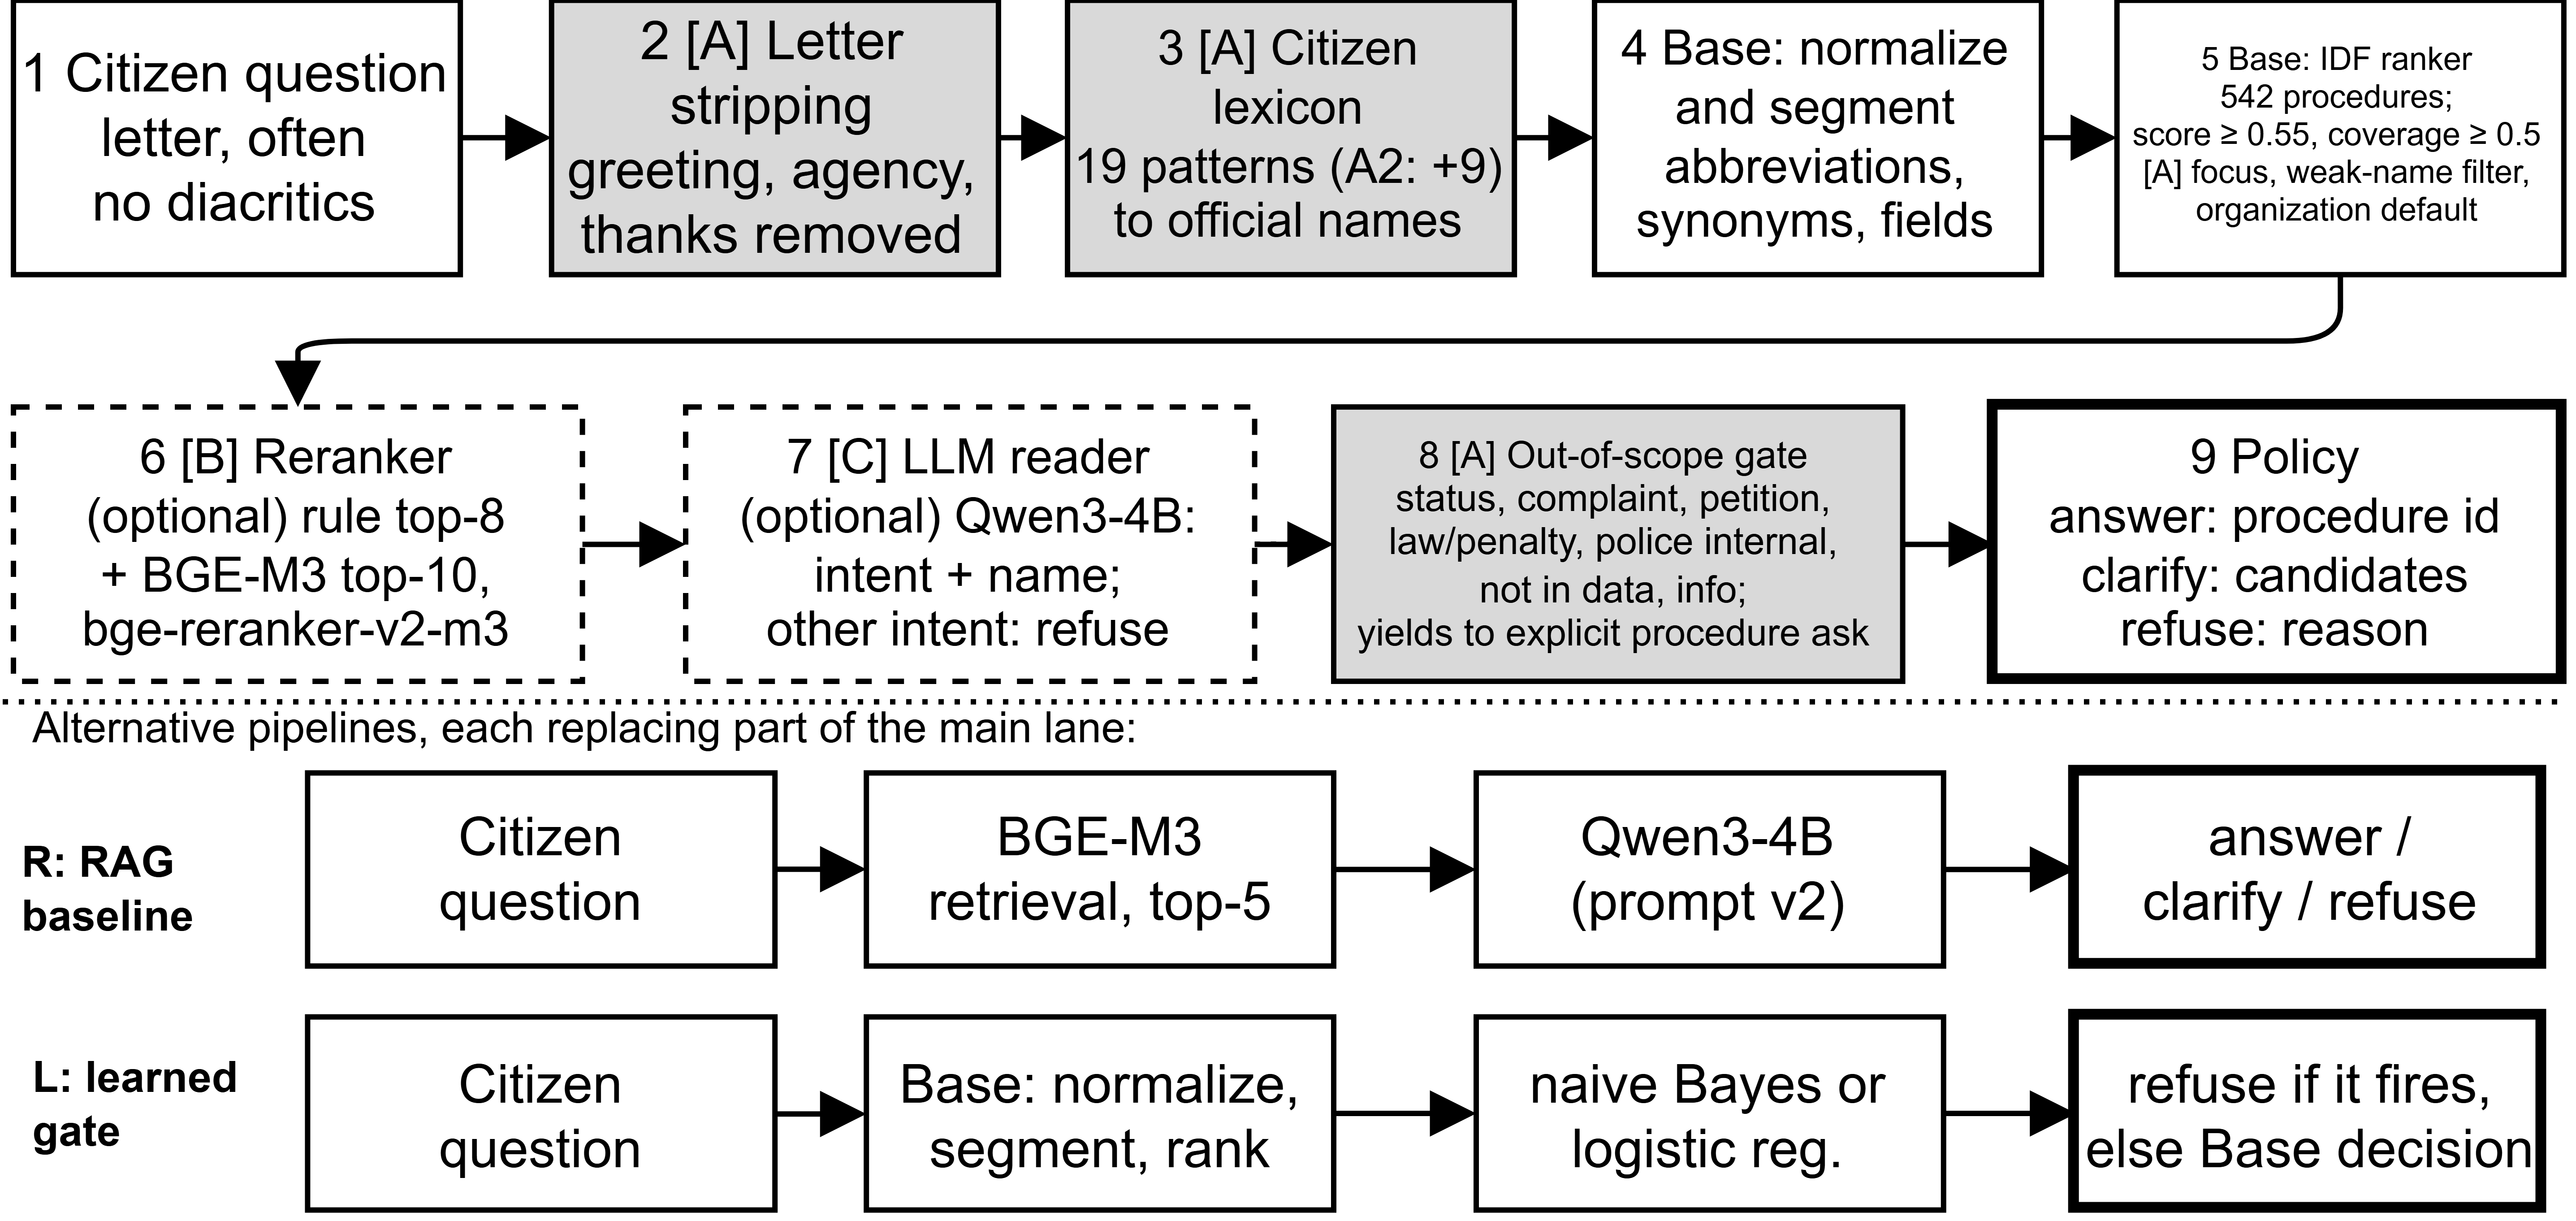
\includegraphics[width=\textwidth]{figures/fig1_pipeline.drawio.png}
\Description{System pipeline diagram. Main lane, first row, left to right: citizen question, letter stripping [A] and citizen lexicon [A] with 19 patterns plus 9 in round two. Base normalizes, segments and IDF-ranks 542 in-scope procedures. Acceptance requires score at least 0.55 and coverage at least 0.5 with rule additions [A]: focus,  weak-namefilter and individual default. Arrow wraps to second row: optional reranker B scores rule top-eight plus ten nearest BGE-M3 candidates using bge-reranker-v2-m3 with thresholds for refuse and swap. Optional reader C (Qwen3-4B) outputs an intent and procedure name; rules rank the name; while other intents yield refusal reasons. Gate A categorizes out-of-scope queries: penalty/law, petition, complaint,status, police internal,absent from data and information requests, yielding to explicit procedural questions. The policy module outputs answer with procedure ID, clarify with candidates or refuse with reason. Below a dotted divider, two alternative pipelines are shown: pipeline R replaces the main lane, retrieving five BGE-M3 procedures and prompting Qwen3-4B v2 for decisions; pipeline L replaces gate A with a learned gate (naive Bayes on n-grams or logistic regression on BGE-M3 embeddings) over base ranking, refusing when triggered or falling back to base decisions. Rule-layer boxes appear gray with [A] tags; optional component are dashed.}
\caption{Configuration legend: base has all switches off; A enables six rule-layer switches (gray boxes tagged [A]); A2 adds the round-2 switch compared with A; B, C are optional hooks (dashed); R and L replace left-side components}\label{fig:pipeline}
\end{figure}

{Rule layer A creates rules  based on errors made by the base system. Each rule has its own switch; disabling all switches exactly reproduces the base system's result on all 313 T1 questions. They were created using the assistant used to label Dev and T1 making them AI assisted. Greetings, organizations addressed and thanks were stripped out, those words otherwise match procedure names.  A citizen lexicon was constructed mapping 19 patterns to their current official names. This includes terms that have been updated by the law on Identification (2023) and Residence Law (2020). Weak names were filtered based on  if  they shared at most three syllables and less than 6\% of a long name. Out of scope rules grouped queries into seven pattern (see Table~\ref{tab:rules}). Petitions, complaints and unavailable procedures were always refused. Queries about status were only overridden by generic processing times. Law, police internal, information were overridden by specific questions about a procedure if it was chosen. Questions $\geq 25$ words were focused so any segments of the question that contain a procedure name would remain. The default organization choice was to choose procedures relating to individuals.}

{In round 2, A2 added one switch, developed after the T1 run to address A's remaining errors on the dev set (595 questions). Additionally, nine lexicon patterns allowed for flexibility with insertions. Explicit citizen requests override procedures inferred from life events. New refusals targeted colloquial status enquiries, officer compensation, personal loans, electricity disputes and deliberate staff delays. Answers followed the common version for all provinces, as specified in the guideline.}

\begin{table}[tb]
\caption{Excerpts from rule layer. Gate: regexes on lowercased diacritic-stripped text. $n$ = pattern count per category. $a$ indicates a question in terms of procedure. A keeps 22 of the 25 override patterns; 3 dropped merely state intention. Only 5 generic processing-time patterns will override status}\label{tab:rules}
\centering\scriptsize
\begin{tabular}{@{}l r p{5.6cm} p{3.6cm}@{}}
\toprule
Gate category & $n$ & Pattern excerpt & Gloss \\
\midrule
status & 16 & \texttt{(?:ma|so) ho so}, \texttt{giay hen}, \texttt{nop} \ldots{} \texttt{chua nhan} & file no., slip, not yet received \\
complaint & 16 & \texttt{khieu nai}, \texttt{to cao}, \texttt{nhung nhieu} & complaint, denunciation, harassment \\
petition & 5 & \texttt{cu tri}, \texttt{kien nghi} & voter, recommendation \\
law / penalty & 27 & \texttt{xu phat}, \texttt{muc phat}, \texttt{vi pham} & sanction, fine level, violation \\
police internal & 4 & staff term \texttt{.\{0,120\}} perk term (2); police-school admission (2) & officer pay, retirement; admission \\
not in data & 35 & \texttt{ly lich tu phap}, \texttt{(?:doi|cap lai|cap|lam) ho chieu} & judicial record, passport \\
info & 14 & \texttt{loi ich}, \texttt{so sanh} & benefits, comparison \\
override & 22 & \texttt{(?:giay to|ho so) (?:gi|nao|\ldots)}, \texttt{le phi}, \texttt{quy trinh} & which papers, fee, process$^a$ \\
\midrule

\bottomrule
\end{tabular}
\end{table}

\subsection{Alternatives}

\emph{Reranker (B).}
{Candidates comprise the top-8 rule rankers and ten nearest neighbors on BGE-M3 ~\cite{chen2024m3}. The bge-reranker-v2-m3 scores them ~\cite{bgererank}. If we receive a score less than a certain threshold then we reject. If a competitor scores higher than our rule choice by a specified amount then they will be chosen instead.}
\emph{LLM reader (C).}
{Qwen3-4B-Instruct-2507 ~\cite{qwen3inst} uses a classify-not-answer prompt with one-line definitions and six team-written examples. It predicts one of six intents: own-file status, procedure, law, complaint or petition, other and police/army internal. For procedure intent, it also extracts a short official name. Name extraction always occurs, but the name returned by C overrides the rule choice only if (1) the rule ranker accepts that name and (2) the rule choice is absent from the ranker's top three. Other intents become refusal reasons. The name-only variant ignores intent.}
\emph{Learned gates (L).}
{These gates were trained post hoc on dev labels: 282 (T1) and 595 (T2). We experimented with two options. One is naive Bayes classifier using word and character n-grams. Other is class-balanced logistic on BGE-M3 embedding. These replace the rule gate in base system.}
\emph{RAG baseline (R).}
{BGE-M3 retrieves the top five in-scope procedures; a 4B model acting as a commune officer answers with a procedure ID, clarifies or refusal. Selected prompt v2 enforces ordered steps: First, refuse non-procedural requests (own-file status, complaint, petition, fine/law or internal). Second, answer when exactly one procedure matches; finally, clarify only when the intended procedure is unclear, otherwise refuse.}

\subsection{Experimental Setup}\label{sec:setup}

{The 13 October 2026 snapshot of the data was used for all runs. We used one laptop with a thermal guard and RTX 4050 NVIDIA GeForce (6 GB). Base, A and A2 are non-LLM based. Ollama served the 4B model with \texttt{Q4\_K\_M} quantization, temperature 0 and JSON-schema output. C had 60-token limit and 20 s timeout. R had 40-token limit and 60 s timeout. Any invalid procedure numbers from R counted as refusals. All thresholds were tuned on dev only. Tuning budgets differed ~\cite{dodge2019}. Rules were tuned extensively. B had a threshold grid and C had one prompt tuned. R had three prompts tuned with v2 chosen on dev (\BA{} 0.445 versus 0.343 and 0.432). L had one threshold and a constant. The software and summaries were created using the assistant in Sect.~\ref{sec:data}. All commands and outputs were committed.}

\section{Results}\label{sec:results}

\subsection{RQ1: Team-Written versus Real Questions}

{The frozen base achieves 77.2\% behavior accuracy (95\% CI: 73--81\%) on 518 team-written questions. In real-world questions, accuracy falls to 56.0\% (50--62\%) on dev and 56.5\% (51--62\%) on T1. \BA{} drops from 0.852 to 0.636 and 0.647, respectively. This decline is mainly due to the difference in question type: must-refuse cases account for 78\% (dev), 79\% (T1) and 92\% (T2) compared with only 11\% of team-written questions. Top-1 accuracy on answerable questions drops from 274/381 (71.9\%) to 7/55 (12.7\%) on dev and 20/59 (33.9\%) on T1. Correct refusals cover only about half of these cases: 116/220 (dev) and 132/248 (T1), versus 52/58 (team-written). On team-written questions, the rule layer shows no net change (+4/-4). Thus, team-written questions hide both the problem and the remedy.}

\subsection{RQ2: The Rule Layer under Declared Comparisons}

{On T1 (Tables~\ref{tab:main} and~\ref{tab:paired}), the rule layer raises \BA{} from 0.647 to 0.814 ($\Delta$ \BA +0.167 [0.095, 0.240]). E2E increases from 19 to 35/59 ($p$ = 0.004). The number of correct refusals increases from 132 to 219/248, while correct answer decisions stay about the same (45 vs 44). The declared round-1 selection A+B over base gains +0.175 [0.104, 0.247]. Both random stratum and MPS rise from 0.512 to 0.859 and 0.618 to 0.875 respectively. Moreover, Binh Dinh also improves from 0.649 to 0.751, which touches zero with its interval [-0.001, 0.206]. Under second-pass labels (91 questions), 24 are gained and 1 is lost.}

{Declared T2 base $\rightarrow$ A2+B comparison raises \BA{} +0.158 [0.009, 0.304], with 129 gains/9 losses. Descriptively, Rule layer A raised refusals (175 $\rightarrow$ 297/335), with 125 gains/5 losses; with $\Delta$ \BA{} = +0.135 [0.033, 0.228], and E2E increases 5 $\rightarrow$ 9/21 but not resolvable ($p$ = 0.125). Round 2 showed no detectable gain: A2+B gained 25 and lost zero behavior decisions against A on dev. On T2, it tied A+B in behavior decisions (+3/-3), with $\Delta$ \BA{} =+0.046 [-0.048, 0.143]. No E2E gain was resolved on T2 (8 versus 10 correct, $p$ = 0.625), and effects of $\pm0.125$ not ruled out, a range as large as the round-1 gain.}

\begin{table}[tb]
\caption{Two test sets evaluated once each  (313 and 363 questions). Ref. shows correct refusals out of 248 (T1) and 335 (T2). E2E count  correct end-to-end answers (denominators 59, 21). Prec. = answer precision (\%). Gate only applies A's gate on base. * post hoc; \textdagger{} added after T1 was opened; -- unrun (A2 developed on T1 questions)}\label{tab:main}
\centering\scriptsize\setlength{\tabcolsep}{3pt}%
\begin{tabular}{@{}lcccccccc@{}}
\toprule
 & \multicolumn{4}{c}{Test 1} & \multicolumn{4}{c}{Test 2} \\
\cmidrule(lr){2-5}\cmidrule(l){6-9}
Configuration & \BA & Ref. & E2E & Prec. & \BA & Ref. & E2E & Prec. \\
\midrule
Always refuse & 0.500 & 248 & 0 & -- & 0.500 & 335 & 0 & -- \\
Base & 0.647 & 132 & 19 & 11.7 & 0.571 & 175 & 5 & 3.0 \\
B: reranker alone & 0.692 & 175 & 21 & 17.9 & -- & -- & -- & -- \\
C: LLM reader alone & 0.785 & 213 & 25 & 30.9 & -- & -- & -- & -- \\
R: RAG, LLM decides$^\dagger$ & 0.489 & 104 & 28 & 43.8 & 0.413 & 197 & 4 & 10.5 \\
L: naive Bayes gate$^*$ & 0.765 & 224 & 14 & 21.9 & 0.579 & 308 & 2 & 6.9 \\
L: embedding gate$^*$ & 0.801 & 225 & 17 & 25.4 & 0.586 & 313 & 2 & 8.0 \\
Gate only$^*$ & 0.770 & 218 & 15 & 20.8 & 0.666 & 287 & 5 & 9.1 \\
\bfseries A: rule layer & \bfseries 0.814 & \bfseries 219 & \bfseries 35 & \bfseries 45.5 & \bfseries 0.705 & \bfseries 297 & \bfseries 9 & \bfseries 19.6 \\
A\,+\,C (intent and name) & 0.817 & 237 & 32 & 58.2 & -- & -- & -- & -- \\
A\,+\,C (name only) & 0.834 & 216 & 39 & 47.0 & -- & -- & -- & -- \\
A\,+\,B (round-1 selection) & 0.823 & 219 & 36 & 46.2 & 0.683 & 298 & 8 & 17.4 \\
A2\,+\,B (round-2 selection) & -- & -- & -- & -- & 0.729 & 297 & 10 & 20.0 \\
\bottomrule
\end{tabular}
\end{table}

\begin{table}[tb]
\caption{Paired differences $X \to Y$. P = primary round 2 comparison (McNemar's test). D = round 1 base--variant comparisons using Wilson intervals (See Table~\ref{tab:main} for other variations). d = descriptive; clar = R's clarification responses: treated as refusals. $\Delta$ \BA{} = paired 95\% bootstrapped confidence intervals after the runs. $m$ = equivalence margin for the 90\% interval, showed only when the 95\% interval includes 0. Behavior and E2E = gains/losses from Y, $p$ = exact McNemar tests}\label{tab:paired}
\centering\scriptsize\setlength{\tabcolsep}{3pt}%
\begin{tabular}{@{}ll c r c l l@{}}
\toprule
Set & X $\rightarrow$ Y & Role & $\Delta$\BA\ [95\% CI] & $m$ & Behavior $+/-$ ($p$) & E2E X$\rightarrow$Y ($+/-$, $p$) \\
\midrule
\bfseries T1 & \bfseries Base $\rightarrow$ A & \bfseries D & $+0.167$ [$+0.095$, $+0.240$] & -- & $+96/{-10}$ ($9\cdot10^{-19}$) & 19$\rightarrow$35 ($+22/{-6}$, 0.004) \\
T1 & Base $\rightarrow$ A\,+\,B & D & $+0.175$ [$+0.104$, $+0.247$] & -- & $+96/{-9}$ ($2\cdot10^{-19}$) & 19$\rightarrow$36 ($+23/{-6}$, 0.002) \\
T1 & A $\rightarrow$ C & d & $-0.029$ [$-0.098$, $+0.038$] & 0.087 & $+28/{-35}$ (0.450) & 35$\rightarrow$25 ($+7/{-17}$, 0.064) \\
T1 & A $\rightarrow$ A\,+\,C (intent) & d & $+0.002$ [$-0.054$, $+0.057$] & 0.049 & $+25/{-10}$ (0.017) & 35$\rightarrow$32 ($+8/{-11}$, 0.648) \\
T1 & A $\rightarrow$ A\,+\,C (name) & d & $+0.019$ [$-0.006$, $+0.051$] & 0.046 & $+4/{-3}$ (1.000) & 35$\rightarrow$39 ($+8/{-4}$, 0.388) \\
T1 & Always refuse $\rightarrow$ R & d & $-0.011$ [$-0.082$, $+0.060$] & 0.071 & -- & -- \\
T1 & A $\rightarrow$ R (clar.\ as ref.) & d & $-0.087$ [$-0.176$, $-0.002$] & -- & $+31/{-39}$ (0.403) & -- \\
\midrule
T2 & A\,+\,B $\rightarrow$ A2\,+\,B & P & $+0.046$ [$-0.048$, $+0.143$] & 0.125 & $+3/{-3}$ (1.000) & 8$\rightarrow$10 ($+3/{-1}$, 0.625) \\
\bfseries T2 & \bfseries Base $\rightarrow$ A2\,+\,B & \bfseries P & $+0.158$ [$+0.009$, $+0.304$] & -- & $+129/{-9}$ ($2\cdot10^{-28}$) & 5$\rightarrow$10 ($+7/{-2}$, 0.180) \\
T2 & A2\,+\,B $\rightarrow$ R & P & $-0.316$ [$-0.427$, $-0.211$] & -- & $+19/{-122}$ ($1\cdot10^{-19}$) & 10$\rightarrow$4 ($+1/{-7}$, 0.070) \\
T2 & Always refuse $\rightarrow$ R & d & $-0.087$ [$-0.175$, $+0.015$] & 0.163 & -- & -- \\
\bottomrule
\end{tabular}
\end{table}

\subsection{RQ3: Alternatives and What the Data Can Detect}

{Alone, the reranker (0.692) and reader (0.785) scored below rule. Compared with A, the reader reduced E2E responses (35$\rightarrow$25); with McNemar ($p=0.064$), while bootstrap CI excluded zero ($\Delta=-0.170$ [$-0.333$, $-0.016$]), without asserting significance. Over rules, reranker gained one correct answer, while reader intent added correct refusal ($p$ = 0.017) but showed no detectable change in \BA{} (within $\pm 0.049$) or E2E. Name-only reached top \BA{} 0.834 (39 E2E responses), differing within $\pm 0.046$ in \BA{} (E2E $p$ = 0.388) and was not chosen by the selection rule.}

{On T1, learned gates showed no detectable difference from the rule gate (Naive Bayes $\pm 0.048$). On T2, learned gates correctly refuse 308 and 313 cases compared (rule gate: 287), improving behavior accuracy post hoc (post hoc tests, $p$ = 0.026 and 0.003). However, they chose answer decision on only 5/21 answerable questions (rules: 10); lowering \BA{}, but not significantly lower.}

{After testing three prompts on dev, the RAG baseline (R) with the selected v2 prompt scored \BA{} of 0.489 (T1) and 0.413 (T2), no better than always-refuse ($\Delta =$ -0.011 [-0.082, 0.060] and -0.087 [-0.175, 0.015], respectively). This was mainly due to clarifications on must-refuse questions (118 on T1; 108 on T2). Treating clarification as refusals raises \BA{} to 0.727 and 0.574, still below the rule layer on T1. Clarification remained hardly evaluated: no T1 setup exceeded one of six cases, while R reached 4/7 on T2 but generated 108 clarifications.}

{At 80\% power (59 answerable on T1 and 21 on T2), only large effects were detectable: $\Delta$ \BA{} = 0.04--0.13 (T1) and 0.13--0.21 (T2). T1 required a 10--15 question E2E difference, while T2 McNemar test required at least 6 discordant pairs in the same direction for $p<0.05$.}

\subsection{RQ4: Deployment Utility}

{Answer precision was 45.5\% for A on T1 and 20.0\% for A2+B on T2. Among A's incorrect answers 29/42 (T1) and 34/37 (T2) were on must-refuse cases; the rule layer reduced these case from 114 to 29 and 153 to 34, respectively (Table~\ref{tab:confusion}). On T2, all configurations had $c^* \leq 0.25$, making always-refuse at least as useful when incorrect answers cost $\geq0.25$ of correct ones. Only A+C gives a value greater than 1 on T1 ($c^* = 1.39$), but in the random stratum it only achieves a value of 0.875, with 7 of 15 answers being correct. In the topical stratum, $c^*$ is achieved by A (1.0) and A+C (1.67) showing that utility depends on traffic composition. No configuration produced more correct than incorrect answers in random traffic. Without stored confidence scores, risk-coverage curves were unavailable, and the protocol prohibited reruns after test-set unblinding.}

\begin{table}[tb]
\caption{Confusion matrices and operating points for each class of gold answers, giving counts of correct procedure / wrong procedure / clarify / refuse. Prec. show the precision of answers (\%), $c^*$ is the cost of incorrect answers when the configuration performs equally well as always-refuse. $U(1)$ is the utility per 100 questions at cost $c=1$, relative to 0 for always-refuse}\label{tab:confusion}
\centering\scriptsize\setlength{\tabcolsep}{3pt}%
\begin{tabular}{@{}llccc r r r@{}}
\toprule
Set & Configuration & gold answer & gold clarify & gold refuse & Prec. & $c^*$ & $U(1)$ \\
\midrule
T1 & Base & 19/26/3/11 & --/4/0/2 & --/114/2/132 & 11.7 & 0.13 & $-39.9$ \\
\bfseries T1 & \bfseries A & \bfseries 35/9/3/12 & \bfseries --/4/0/2 & \bfseries --/29/0/219 & \bfseries 45.5 & \bfseries 0.83 & \bfseries\boldmath $-2.2$ \\
T1 & A\,+\,B & 36/9/2/12 & --/4/0/2 & --/29/0/219 & 46.2 & 0.86 & $-1.9$ \\
T1 & A\,+\,C (intent) & 32/8/1/18 & --/4/1/1 & --/11/0/237 & 58.2 & 1.39 & $+2.9$ \\
T1 & R & 28/5/23/3 & --/5/1/0 & --/26/118/104 & 43.8 & 0.78 & $-2.6$ \\
T1 & L embedding & 17/24/2/16 & --/3/0/3 & --/23/0/225 & 25.4 & 0.34 & $-10.5$ \\
\midrule
T2 & Base & 5/8/2/6 & --/1/1/5 & --/153/7/175 & 3.0 & 0.03 & $-43.3$ \\
T2 & A & 9/2/2/8 & --/1/1/5 & --/34/4/297 & 19.6 & 0.24 & $-7.7$ \\
T2 & A2\,+\,B & 10/2/2/7 & --/2/0/5 & --/36/2/297 & 20.0 & 0.25 & $-8.3$ \\
T2 & R & 4/1/13/3 & --/3/4/0 & --/30/108/197 & 10.5 & 0.12 & $-8.3$ \\
T2 & L embedding & 2/3/2/14 & --/0/1/6 & --/20/2/313 & 8.0 & 0.09 & $-5.8$ \\
\bottomrule
\end{tabular}
\end{table}

\section{Discussion and Limitations}\label{sec:discussion}

\subsubsection{What the Protocol Caught.}

{Without the protocol, two wrong conclusions would stand: the base system works (team-written set) and the second rule round helps (dev). A2+B changed A's decision or top procedure at similar rates: 6.2\% on dev, 5.2\% on T2. Strictly, with answers credited only for the right procedure, dev moved +30/$-$0 and T2 +4/$-$4. By behavior, the moves were +25/$-$0 and +4/$-$4. This pattern suggests rules tuned to particular phrasings. Labels produced by a different model and the small answer class may also contribute.}

\subsubsection{What Remains.}

{On T1, A missed 24 answers: two sets of 12. One set was refused, 8 at the gate, including 4 where the base system's top procedure was right. A's five candidates lacked the correct procedure for 7 others. Our results suggest against unsupervised answering: an officer confirms replies, or the system answers only when confident~~\cite{geifman2017}.
}

\subsubsection{Limitations.}

(i)~{The study covers a single domain, a single language and a single data snapshot.} 
(ii)~{The test sets contain 59 and 21 answer but only 6 and 7 clarify questions, so only large differences are detectable. Clarification is part of the task yet hardly evaluated, so we draw no conclusion about it.} 
(iii)~{Our labels had LLM help: for dev and T1, the rule-writing assistant produced them after reading every T1 question. Its notion of scope may thus be built into the gate~~\cite{pangakis2023,reiss2023}. On T2, labeled without it, the gain persists (+125/$-$5). Circularity thus seems an unlikely full account, though shared guideline scope cannot be excluded. Until humans label independently, gains hold only under our guideline.} 
(iv)~{Neither data source is a commune office. Categories such as police-internal questions are likely rarer at a commune office. The share of questions to refuse there is unknown.} 
(v)~{Our locks are commits in a private development repository, so they carry no external timestamps.
} 
(vi)~{The rules received far more tuning effort than other components, so our claims about the reranker (B), LLM reader (C), learned gates (L) and RAG baseline (R) concern these lightly tuned baselines only. We did not run a fine-tuned PhoBERT gate~~\cite{nguyen2020phobert} or a few-shot or calibrated LLM gate. Ablations and learned gates are post hoc.} 
(vii)~{The LLM components use a single run at
temperature 0 and one quantized model.} 
(viii)~{We report no risk-coverage curve, and the source datasets state no license.}

\section{Conclusion}\label{sec:conclusion}

{We investigated an administrative assistant limited to commune-level procedures. The main challenge in real-world question is deciding whether to answer. We evaluated the AI-assisted rule layer under a locked, run-once protocol. Correct E2E answers nearly double on T1 (19 to 35/59). The refusal improvement was maintained on T2. Round 2 improved dev result but showed no detectable gain on unseen data. None of the four alternatives detectably improved either \BA{} or E2E over the rule layer.}

\subsubsection{Ethics and Data Availability.}

{Procedure records are publicly available and does not contain any private data. We took questions from public datasets and cards which did not have license details. Any personal data was masked before labeling. This paper contains no names / identifiers and no human-participant data collected. Question content will not be redistributed. We release code, IDs, source pointers of 958 labeled questions, SHA-256 hashes of the locked test files, labels, and per-question run decisions at \url{https://github.com/NCKH-LongT/chatbot-thutuc-g7/tree/main/Code}.}

{Before publication, we revised five commit messages without altering the trees or dates. Old-to-new hashes mapping is in the repository.}
{\emph{Use of AI.} The authors wrote the paper without generative AI assistance. Claude Opus 5.5 (Anthropic) was used only to build the software including the rule layer, summarize the test results, and support labeling (Sect.~\ref{sec:data}), while Gemini 4 Argon helped with labeling. The authors take full responsibility for the content.}

\begin{credits}
\subsubsection{\ackname} 
{No external funding was received.}

\subsubsection{\discintname} 
{The authors declare no competing interests.}
\end{credits}

\nocite{dvcportal,kaplan2026,samson2026,wen2025,kamath2020,larson2019,phamduy2023,dwork2015,gorman2019,nguyen2020phobert,vigptqa2023,hien2025,alqac2021,elyaniv2010,geifman2017,chow1970,hendrycks2017,aliannejadi2019,lewis2020,asai2024,rebedea2023,chiticariu2013,vanmiltenburg2021,dodge2019,gilardi2023,pangakis2023,reiss2023,hfdvc,hfmps,cohen1960,brodersen2010,wilson1927,mcnemar1947,dietterich1998,connor1987,schuirmann1987,chen2024m3,bgererank,qwen3inst}
\bibliographystyle{splncs04}
\bibliography{refs}

\end{document}
